
% spellcheck: ok
% mikes: ok

\chapter{Arguments from Probability Models}{}{}
\label{ch:probability}

\index{data analysis!probability models|(} 
\index{probability models|(} 
\index{distributions|(} 

% probabilistic reasoning
% stochastic
% random
% probability
% non-deterministic
% uncertainty

\Fint{When modeling systems that exhibit some form of randomness, the
challenge in the modeling} process is to find a way to handle the
resulting uncertainty. We don't know for sure what the system will
do---there is a range of outcomes, each of which is more or less
likely, according to some probability distribution. Occasionally, it is
possible to work out the exact probabilities for all possible events;
however, this quickly becomes very difficult, if not impossible, as we
go from simple (and possibly idealized systems) to real applications.
We need to find ways to simplify life!

In this chapter, I want to take a look at some of the ``standard''
probability models that occur frequently in practical problems. I
shall also describe some of their properties that make it possible to
reason about them without having to perform explicit calculations for
all possible outcomes. We will see that we can reduce the behavior of
many random systems to their ``typical'' outcome and a narrow range
around that.

This is true for many situations but not for all! Systems
characterized by power-law distribution functions can \emph{not} be
summarized by a narrow regime around a single value, and you will
obtain highly misleading (if not outright wrong) results if you try to
handle such scenarios with standard methods. It is therefore important
to recognize this kind of behavior and to choose appropriate
techniques.


% ============================================================
\section{The Binomial Distribution and Bernoulli Trials}

\index{probability models!Binomial distribution and Bernoulli trials|(} 
\index{Binomial distribution and Bernoulli trials|(}
\index{distributions!Binomial distribution and Bernoulli trials|(} 
 
Bernoulli trials are random trials that can have only two outcomes,
commonly called Success and Failure. Success occurs with\vadjust{\pagebreak} probability
$p$, and Failure occurs with probability $1-p$. We further assume that
successive trials are independent and that the probability parameter
$p$ stays constant throughout.

Although this description may sound unreasonably limiting, in fact
many different processes can be expressed in terms of Bernoulli
trials.  We just have to be sufficiently creative when defining the
class of events that we consider ``Successes.'' A few examples:

\begin{itemize}
\item Define Heads as Success in $n$ successive tosses of a fair coin.
  In this case, $p=1/2$.
\item Using fair dice, we can define getting an ``ace'' as Success and
  all other outcomes as Failure. In this case, $p=1/6$.
\item We could just as well define \emph{not} getting an ``ace'' 
  as Success. In this case, $p=5/6$.
\item Consider an urn that contains $b$ black tokens and $r$ red
  tokens. If we define drawing a red token as Success, then repeated
  drawings (with replacement!) from the urn constitute Bernoulli
  trials with $p = r/(r+b)$.
\item Toss two identical coins and define obtaining two Heads as
  Success. Each toss of the two coins \emph{together} constitutes a
  Bernoulli trial with $p=1/4$.
\end{itemize}

As you can see, the restriction to a binary outcome is not really
limiting: even a process that naturally has more than two possible
outcomes (such as throwing dice) can be cast in terms of Bernoulli
trials if we restrict the definition of Success appropriately.
Furthermore, as the last example shows, even combinations of events
(such as tossing two coins or, equivalently, two successive tosses of
a single coin) can be expressed in terms of Bernoulli trials.

The restricted nature of Bernoulli trials makes it possible to derive
some exact results (we'll see some in a moment).  More importantly,
though, the abstraction forced on us by the limitations of Bernoulli
trials can help to develop simplified conceptual models of a random
process.

\subsection{Exact Results}

The central formula for Bernoulli trials gives the \emph{probability
  of observing $k$ Successes in $N$ trials with Success probability
  $p$}, and it is also known as the \emph{Binomial distribution} (see
Figure \ref{fig:binomial}):
%
\[
P(k, N; p) = \binom{N}{k} p^k (1-p)^{N-k}
\]
%
This should make good sense: we need to obtain $k$ Successes, each
occurring with probability $p$, and $N-k$ Failures, each occurring
with probability $1-p$. The term:
%
\[
\binom{N}{k} = \frac{N!}{k! (N-k)!}
\]
%
consisting of a \emph{binomial coefficient} is combinatorial in
nature: it gives the number of distinct arrangements for $k$ successes\vadjust{\pagebreak}
and $N-k$ failures. (This is easy to see. There are $N!$ ways to
arrange $N$ \emph{distinguishable} items: you have $N$ choices for the
first item, $N-1$ choices for the second, and so on. However, the $k$
Successes are indistinguishable from each other, and the same is true
for the $N-k$ Failures. Hence the total number of arrangements is
reduced by the number of ways in which the Successes can be
rearranged, since all these rearrangements are identical to each
other. With $k$ Successes, this means that $k!$ rearrangements are
indistinguishable, and similarly for the $N-k$ failures.) Notice that
the combinatorial factor does not depend on $p$.

\begin{figure}
\centerline{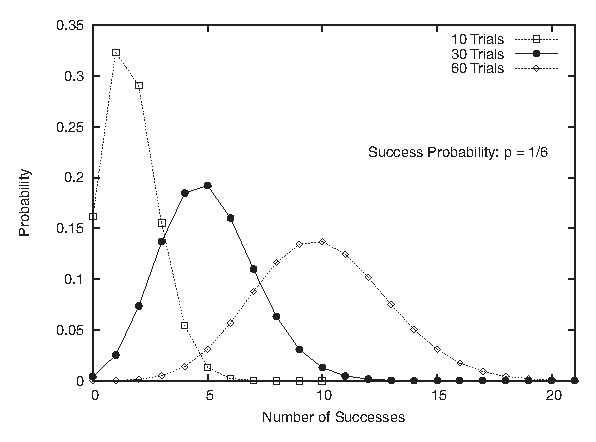
\includegraphics{img/binomial}}
  \caption{The Binomial distribution: the probability of obtaining $k$
    Successes in $N$ trials with Success probability $p$.}
  \label{fig:binomial}
\end{figure}

This formula gives the probability of obtaining a specific number $k$
of Successes. To find the expected number of Successes $\mu$ in $N$
Bernoulli trials, we need to average over all possible outcomes:
%
\begin{align*}
\mu & = \sum_k^N k \, P(k, N; p) \\
    & = N p
\end{align*}
%
This result should come as no surprise. We use it intuitively
whenever we say that we expect ``about five Heads in ten tosses of
fair coin'' ($N=10$, $p=1/2$) or that we expect to obtain ``about
ten aces in sixty tosses of a fair die'' ($N=60$, $p=1/6$).

Another result that can be worked out exactly is the standard
deviation:\index{standard deviation}
%
\[
\sigma = \sqrt{ N p ( 1 - p ) }
\]
%
The standard deviation gives us the range over which we expect
the outcomes to vary. (For example, assume that we perform $m$
experiments, each consisting of $N$ tosses of a fair coin.
The expected number of Successes in each experiment is $N p$,
but of course we won't obtain exactly this number in each 
experiment. However, over the course of the $m$ experiments,
we expect  to find the number of Successes in the majority of
them to lie between $N p - \sqrt{N p (1 - p)}$ and
$N p + \sqrt{N p (1 - p)}$).

Notice that $\sigma$ grows more slowly with the number of trials than
does $\mu$ ($\sigma \sim \sqrt{N}$ versus $\mu \sim N$). The relative
width of the outcome distribution therefore shrinks as we conduct more
trials.

\subsection{Using Bernoulli Trials to Develop Mean-Field Models}

\index{mean-field models} 
\index{Bernoulli trials, mean-field models} 

The primary reason why I place so much emphasis on the concept of
Bernoulli trials is that it lends itself naturally to the development
of mean-field models (see Chapter \ref{ch:scaling}). Suppose we try to
develop a model to predict the staffing level required for a call
center to deal with customer complaints. We know from experience that
about one in every thousand orders will lead to a complaint (hence
$p=1/1000$). If we shipped a million orders a day, we could use the
Binomial distribution to work out the probability to receive $1, 2, 3,
\dots, \text{999,999}, \text{1,000,000}$ complaints a day and then
work out the required staffing levels accordingly---a daunting task!
But in the spirit of mean-field theories, we can cut through the
complexity by realizing that we will receive ``about $N p =
\text{1,000}$'' complaints a day. So rather than working with each
possible outcome (and its associated probability), we limit our
attention to a single \emph{expected} outcome. (And we can now proceed
to determine how many calls a single person can handle per day to find
the required number of customer service people.) We can even go a step
further and incorporate the uncertainty in the number of complaints by
considering the standard deviation, which in this example comes out to
$\sqrt{N p (1-p)} \approx \sqrt{1000} \approx 30$. (Here I made use of
the fact that $1-p$ is very close to $1$ for the current value of
$p$.) The spread is small compared to the expected number of calls,
lending credibility to our initial approximation of replacing the full
distribution with only its expected outcome. (This is a demonstration
for the observation we made earlier that the width of the resulting
distribution grows much more slowly with $N$ than does the expected
value itself. As $N$ gets larger, this effect becomes more drastic,
which means that mean-field theory gets \emph{better} and more
reliable the more urgently we need it! The tough cases can be
situations where $N$ is of moderate size---say, in the range of $10,
\dots, 100$. This size is too large to work out all outcomes exactly
but not large enough to be safe working only with the expected
values.)

Having seen this, we can apply similar reasoning to more general
situations. For example, notice that the number of orders shipped each
day will probably not equal exactly one million---instead, it will be
a random quantity itself. So, by using $N = \text{1,000,000}$ we have
employed the mean-field idea already.  It should be easy to generalize
to other situations from here.

\index{probability models!Binomial distribution and Bernoulli trials|)} 
\index{Binomial distribution and Bernoulli trials|)}
\index{distributions!Binomial distribution and Bernoulli trials|)} 

% ============================================================
\section{The Gaussian Distribution and the Central Limit Theorem}

\index{probability models!Gaussian Distribution and the Central Limit Theorem|(}
\index{Gaussian distribution (Gaussian function)!Central Limit Theorem|(}  
\index{Central Limit Theorem!Gaussian Distribution|(}


Probably the most ubiquitous formula in all of probability theory
and statistics is:
%
\[
p(x; \mu, \sigma ) = \frac{1}{\sqrt{2 \pi} \sigma} \,
                     e^{-\frac{1}{2} \paren{\frac{x-\mu}{\sigma}}^2}
\]
%
This is the formula for the Gaussian (or \emph{Normal}) probability
density. This is the proverbial ``Bell Curve.'' (See Figure
\ref{fig:probgaussian} and Appendix \ref{app:calculus} for additional
details.)

\begin{figure}
\centerline{ 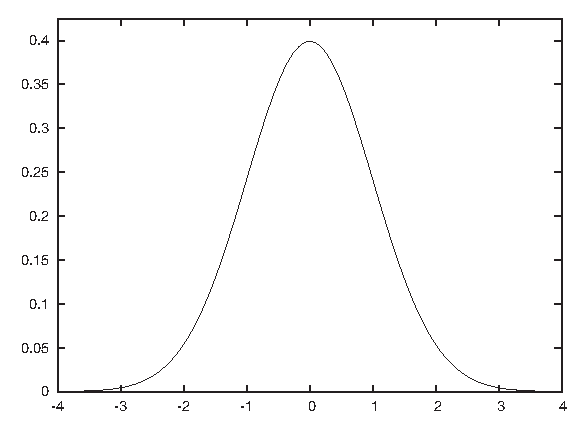
\includegraphics{img/probgaussian}}
  \caption{The Gaussian probability density.}
  \label{fig:probgaussian}
\end{figure}

Two factors contribute to the elevated importance of the Gaussian
distribution: on the foundational side, the Central Limit Theorem
guarantees that the Gaussian distribution will arise naturally
whenever we take averages (of almost anything). On the sheerly
practical side, the fact that we can actually explicitly work out most
integrals involving the Gaussian means that such expressions make good
building blocks for more complicated theories.


\subsection{The Central Limit Theorem}

Imagine you have a source of data points that are distributed
according to some common distribution. The data could be numbers drawn
from a uniform random-number generator, prices of items in a store, or
the body heights of a large group of people.

Now assume that you repeatedly take a sample of $n$ elements from the
source ($n$ random numbers, $n$ items from the store, or measurements\vadjust{\pagebreak}
for $n$ people) and form the total sum of the values. You can also
divide by $n$ to get the average. Notice that these sums (or averages)
are random quantities themselves: since the points are drawn from a
random distribution, their sums will also be random numbers.

Note that we don't necessarily know the distributions from which the
original points come, so it may seem it would be impossible to say
anything about the distribution of their sums. Surprisingly, the
opposite is true: we can make very precise statements about the form
of the distribution according to which the sums are distributed. This
is the content of the Central Limit Theorem.

The \emph{Central Limit Theorem} states that the sums of a bunch of
random quantities will be distributed according to a Gaussian
distribution. This statement is not strictly true; it is only an
approximation, with the quality of the approximation improving as more
points are included in each sample (as $n$ gets larger, the
approximation gets better). In practice, though, the approximation is
excellent even for quite moderate values of $n$.

This is an amazing statement, given that we made no assumptions
whatsoever about the original distributions (I will qualify this in a
moment): it seems as if we got something for nothing! After a moment's
thought, however, this result should not be so surprising: if we take
a single point from the original distribution, it may be large or it
may be small---we don't know. But if we take many such points, then
the highs and the lows will balance each other out ``on average.''
Hence we should not be too surprised that the distribution of the sums
is a \emph{smooth} distribution with a \emph{central peak}. It is,
however, not obvious that this distribution should turn out to be the
Gaussian specifically.

We can now state the Central Limit Theorem formally. \textit{Let
$\braces{x_i}$ be a sample of size $n$, having the following properties:
\begin{enumerate}
\item[\rm 1.] All $x_n$ are mutually independent.
\item[\rm 2.] All $x_n$ are drawn from a common distribution.
\item[\rm 3.] The mean $\mu$ and the standard deviation $\sigma$ for the 
  distribution of the individual data points $x_i$ are finite.
\end{enumerate}
Then the sample average $\frac{1}{n} \sum_i^n x_i$ is distributed
according to a Gaussian with mean $\mu$ and standard deviation
$\sigma/\sqrt{n}$. The approximation improves as the sample size $n$
increases.} In other words, the probability of finding the value $x$
for the sample mean $\frac{1}{n} \sum_i x_i$ becomes Gaussian as $n$
gets large:
%
\[
P\paren{ \frac{1}{n} \sum_i^n x_i = x }
\to
\frac{1}{\sqrt{2 \pi}} \frac{\sqrt{n}}{\sigma} 
  \exp \paren{-\frac{1}{2} \paren{ \frac{x-\mu}{\sigma/\sqrt{n}} }^2 }
\]
%
% Larsen/Marx p302; green Chatfield p112-114; 

Notice that, as for the binomial distribution, the width of the
resulting distribution of the average is smaller than the width of the
original distribution of the individual data points.  This aspect of
the Central Limit Theorem is the formal justification for the common
practice to ``average out the noise'': no matter how widely the
individual data points scatter, their averages will scatter less.

On the other hand, the reduction in width is not as fast as one might
want: it is not reduced linearly with the number $n$ of points in the
sample but only by $\sqrt{n}$. This means that if we take 10 times as
many points, the scatter is reduced to only $1/\sqrt{10} \approx \text{30
  percent}$ of its original value.  To reduce it to 10 percent, we
would need to increase the sample size by a factor of $100$. That's a
lot!

Finally, let's take a look at the Central Limit Theorem in action.
Suppose we draw samples from a uniform distribution that takes on the
values $1, 2, \dots, 6$ with equal probability---in other words,
throws of a fair die. This distribution has mean $\mu = 3.5$ (that's
pretty obvious) and standard deviation $\sigma = \sqrt{(6^2-1)/12}
\approx 1.71$ (not as obvious but not terribly hard to work it out, or
you can look it up).

We now throw the die a certain number of times and evaluate the
average of the values that we observe. According to the Central Limit
Theorem, these averages should be distributed according to a Gaussian
distribution that becomes narrower as we increase the number of throws
used to obtain an average. To see the distribution of values, we
generate a histogram (see Chapter \ref{ch:univariate}). I use 1,000
``repeats'' to have enough data for a histogram. (Make sure you
understand what is going on here: we throw the die a certain number of
times and calculate an average based on those throws; and this entire
process is repeated 1,000 times.)

The results are shown in Figure \ref{fig:cltinaction}. In the
upper-left corner we have thrown the die only once and thus form the
``average'' over only a single throw. You can see that all of the
possible values are about equally likely: the distribution is uniform.
In the upper-right corner, we throw the dice \emph{twice} every time
and form the average over both throws. Already a central tendency in
the distribution of the \emph{average} of values can be observed!  We
then continue to make longer and longer averaging runs. (Also shown is
the Gaussian distribution with the appropriately adjusted width:
$\sigma/\sqrt{n}$, where $n$ is the number of throws over which we
form the average.)

I'd like to emphasize two observations in particular. First, note how
quickly the central tendency becomes apparent---it only takes
averaging over two or three throws for a central peak to becomes
established. Second, note how well the properly scaled Gaussian
distribution fits the observed histograms. This is the Central Limit
Theorem in action.

\begin{figure}
\centerline{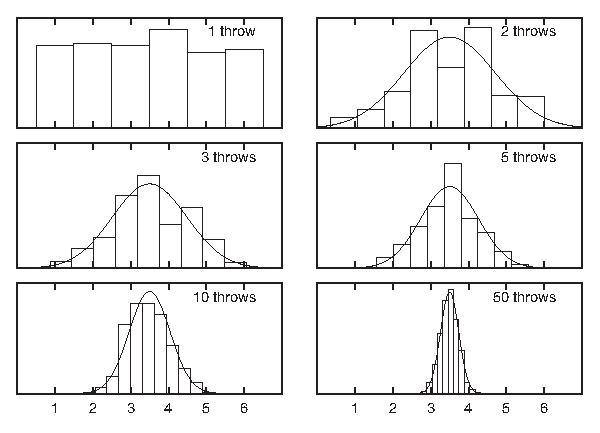
\includegraphics{img/cltinaction}}
  \caption{The Central Limit Theorem in action. Distribution of the
    average number of points when throwing a fair die several times.
    The boxes show the histogram of the value obtained; the
    line shows the distribution according to the Central Limit
    Theorem.}
  \label{fig:cltinaction}
\end{figure}


\subsection{The Central Term and the Tails}

The most predominant feature of the Gaussian density function is the
speed with which it~falls to zero as $\abs{x}$ (the absolute value of
$x$---see Appendix \ref{app:calculus}) becomes large. It is worth~looking at some numbers to
understand just how quickly it does decay. For\break $x=2$, the standard Gaussian with zero mean
and unit variance is approximately $p(2,0,1) = 0.05\dots$. For $x=5$, it is already on the
order of $10^{-6}$; for $x=10$ it's about $10^{-22}$; and not much
further\vadjust{\pagebreak} out, at $x=15$, we find $p(15,0,1) \approx 10^{-50}$.  One
needs to keep this in perspective: the age of the universe is
currently estimated to be about 15 billion years, which is about $4
\cdot 10^{17}$ seconds. So, even if we had made \emph{a thousand
  trials per second since the beginning of time}, we would still not
have found a value as large or larger than $x=10$!

Although the Gaussian is defined for all $x$, its weight is so
strongly concentrated within a finite, and actually quite small,
interval (about $[-5,5]$) that values outside this range will not
occur.  It is not just that only one in a million events will deviate
from the mean by more than 5 standard deviations: the decline
continues, so that fewer than one in $10^{22}$ events will deviate by
more than 10 standard deviations. Large outliers are not just
rare---they don't happen!

This is both the strength and the limitation of the Gaussian model:
\emph{if} the Gaussian model applies, then we know that all variation
in the data will be relatively small and therefore ``benign.'' At the
same time, we know that for some systems, large outliers do occur in
practice. This means that, for such systems, the Gaussian model
\emph{and theories based on it} will not apply, resulting in bad
guidance or outright wrong results. (We will return to this problem
shortly.)


\subsection{Why Is the Gaussian so Useful?}

It is the combination of two properties that makes the Gaussian
probability distribution so common and useful: because of the Central
Limit Theorem, the\vadjust{\pagebreak} Gaussian distribution will occur whenever we we
dealing with averages; and because so much of the Gaussian's weight is
concentrated in the central region, almost any expression can be
approximated by concentrating only on the central region, while
largely disregarding the tails.

As we will discuss in Chapter \ref{ch:statistics} in more detail, the
first of these two arguments has been put to good use by the creators
of classical statistics: although we may not know anything about the
distribution of the actual data points, the Central Limit Theorem
enables us to make statements about their averages. Hence, if we
concentrate on estimating the sample \emph{average} of any quantity,
then we are on much firmer ground, theoretically. And it is impressive
to see how classical statistics is able to make rigorous statements
about the extent of confidence intervals for parameter estimates while
using almost no information beyond the data points themselves!  I'd
like to emphasize these two points again: through clever application
of the Central Limit Theorem, classical statistics is able to give
\emph{rigorous} (not just intuitive) bounds on estimates---and it can
do so without requiring detailed knowledge of (or making additional
assumptions about) the system under investigation. This is a
remarkable achievement!

The price we pay for this rigor is that we lose much of the richness
of the original data set: the distribution of points has been boiled
down to a single number---the average.

The second argument is not so relevant from a conceptual point, but
it is, of course, of primary practical importance: we can actually do
many integrals involving Gaussians, either exactly or in very good
approximation. In fact, the Gaussian is so convenient in this regard
that it is often the first choice when an integration kernel is needed
(we have already seen examples of this in Chapter \ref{ch:univariate},
in the context of kernel density estimates, and in Chapter
\ref{ch:timeseries}, when we discussed the smoothing of a time
series).

\subsection{Optional: Gaussian Integrals}

\index{integrals!Gaussian integrals}
 
The basic idea goes like this: we want to evaluate an integral of
the form:
%
\[
\int\! f(x) e^{-x^2/2} \rms{x}
\]
%
We know that the Gaussian is peaked around $x=0$, so that only nearby
points will contribute significantly to the value of the integral.  We
can therefore expand $f(x)$ in a power series for small $x$. Even if
this expansion is no good for large $x$, the result will not be
affected significantly because those points are suppressed by the
Gaussian. We end up with a series of integrals of the form
%
\[
a_n \int\! x^n e^{-x^2/2} \rms{x}
\]
%
which can be performed exactly. (Here, $a_n$ is the expansion
coefficient from the expansion of $f(x)$.)

We can push this idea even further. Assume that the kernel is not
exactly Gaussian but is still strongly peaked:
%
\[
\int\! f(x) e^{-g(x)} \rms{x}
\]
%
where the function $g(x)$ has a minimum at some location (otherwise,
the kernel would not have a peak at all). We can now expand $g(x)$
into a Taylor series around its minimum (let's assume it is at $x=0$),
retaining only the first two terms: $g(x) \approx g(0) +
g^{\prime\prime}(0) x^2/2 + \dotsb$. The linear term vanishes because
the first derivative $g^\prime$ must be zero at a minimum.  Keeping in
mind that the first term in this expansion is a constant not depending
on $x$, we have transformed the original integral to one of Gaussian
type:
%
\[
e^{-g(0)} \int\! f(x) e^{-g^{\prime\prime}(0) \, x^2/2} \rms{x}
\]
%
which we already know how to solve. 

This technique goes by the name of \emph{Laplace's method} (not to be
confused with ``Gaussian integration,'' which is something else
entirely).


\subsection{Beware: The World Is Not Normal!}

Given that the Central Limit Theorem is a rigorously proven theorem,
what could possibly go wrong? After all, the Gaussian distribution
guarantees the absence of outliers, doesn't it?  Yet we all know that
unexpected events \emph{do} occur.

There are two things that can go wrong with the discussion so far:

\begin{itemize}
\item The Central Limit Theorem only applies to sums or averages of
  random quantities but not necessarily to the random quantities
  themselves.  The distribution of individual data points may be quite
  different from a Gaussian, so if we want to reason about
  individual events (rather than about an aggregate such as their
  average), then we may need different methods.
  For example, although the \emph{average} number of items in a
  shipment may be Gaussian distributed around a typical value of three
  items per shipment, there is no guarantee that the actual
  distribution of items per shipment will follow the same
  distribution. In fact, the distribution will probably be
  geometrical, with shipments containing only a single item being much
  more common than any other shipment size.

\item More importantly, the Central Limit Theorem \emph{may not
    apply}.  Remember the three conditions listed as requirements for
  the Central Limit Theorem to hold? Individual events must be
  independent, follow the same distribution, and must have a finite mean
  and standard deviation.  As it turns out, the first and second of
  these conditions can be weakened (meaning that individual events can
  be somewhat correlated and drawn from slightly different
  distributions), but the third condition \emph{cannot} be weakened:
  individual events \emph{must} be drawn from a distribution of finite
  width.

  Now this may seem like a minor matter: surely, all distributions
  occurring in practice are of finite width, aren't they? As it turns
  out, the answer is \emph{no}! Apparently ``pathological''
  distributions of this kind are much more common in real life than
  one might expect. Such distributions follow \emph{power-law}
  behavior, and they are the topic of the next section.
\end{itemize}

\index{probability models!Gaussian Distribution and the Central Limit Theorem|)}
\index{Gaussian distribution (Gaussian function)!Central Limit Theorem|)}   
\index{Central Limit Theorem!Gaussian Distribution|)}

% ============================================================
\section{Power-Law Distributions and Non-Normal Statistics}

\index{probability models!power-law distributions|(} 
\index{power-law distributions!non-normal statistics|(} 
\index{non-normal statistics and power-law distributions|(}
\index{distributions!power-law distributions|(}
  
Let's start with an example. Figure \ref{fig:webvisits1} shows a
histogram for the number of visits per person that a sample of
visitors made to a certain website over one month. Two things stand
out: the huge number of people who made a handful of visits (fewer
than 5 or 6) and, at the other extreme, the huge number of visits
that a few people made. (The heaviest user made 41,661 visits: that's
about one per minute over the course of the month---probably a bot or
monitor of some sort.)

This distribution looks nothing like the ``benign'' case in Figure
\ref{fig:probgaussian}. The distribution in Figure
\ref{fig:webvisits1} is not merely skewed---it would be no
exaggeration to say that it consists \emph{entirely} of outliers!
Ironically, the ``average'' number of visits per person---calculated
naively, by summing the visits and dividing by the number of unique
visitors---equals 26 visits per person. This number is clearly not
representative of anything: it describes neither the huge majority of
light users on the lefthand side of the graph (who made one or two
visits), nor the small group of heavy users on the right. (The
standard deviation is $\pm 437$, which clearly suggests that something
is not right, given that the mean is 26 and the number of visits must
be positive.)

This kind of behavior is typical for distributions with so-called
\emph{fat} or \emph{heavy tails}. In contrast to systems ruled by a
Gaussian distribution or another distribution with short tails, data
values are not effectively limited to a narrow domain. Instead, we can
find a nonnegligible fraction of data points that are very far away
from the majority of points.

Mathematically speaking, a distribution is heavy-tailed if it falls to
zero much slower than an exponential function.  Power laws ({\it i.e.}, 
functions that behave as $\sim 1/x^\beta$ for some exponent $\beta>0$)
are usually used to describe such behavior.

In Chapter \ref{ch:bivariate}, we discussed how to recognize power
laws: data points falling onto a straight line on a double logarithmic
plot.  A double logarithmic plot of the data from Figure
\ref{fig:webvisits1} is shown in Figure \ref{fig:webvisits2}, and we
see that eventually (\ie, for more than five visits per person), the
data indeed follows a power law (approximately $\sim x^{-1.9}$). On
the lefthand side of Figure \ref{fig:webvisits2} (\ie, for few visits
per person), the behavior is different. (We will come back to this
point later.)

\begin{figure}
\centerline{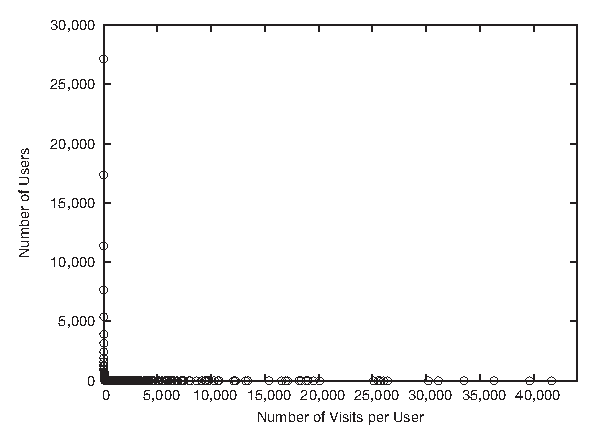
\includegraphics{img/webvisits1}}
  \caption{A histogram of the number of visitors who made $x$ number
    of visits to a certain website. Note the extreme skewness of the
    distribution: most visitors made one or two visits, but a few made
    tens of thousands of visits.}
  \label{fig:webvisits1}
\end{figure}

Power-law distributions like the one describing the data set in in
Figures \ref{fig:webvisits1} and \ref{fig:webvisits2} are surprisingly
common. They have been observed in a number of different (and often
colorful) areas: the frequency with which words\vadjust{\pagebreak} are used in texts, the
magnitude of earthquakes, the size of files, the copies of books
sold, the intensity of wars, the sizes of sand particles and solar
flares, the population of cities, and the distribution of wealth.
Power-law distributions go by different names in different
contexts---you will find them referred to as ``Zipf'' of ``Pareto''
distributions, but the mathematical structure is always the same.  The
term ``power-law distribution'' is probably the most widely accepted,
general term for this kind of heavy-tailed distribution.
 
\begin{figure}
\centerline{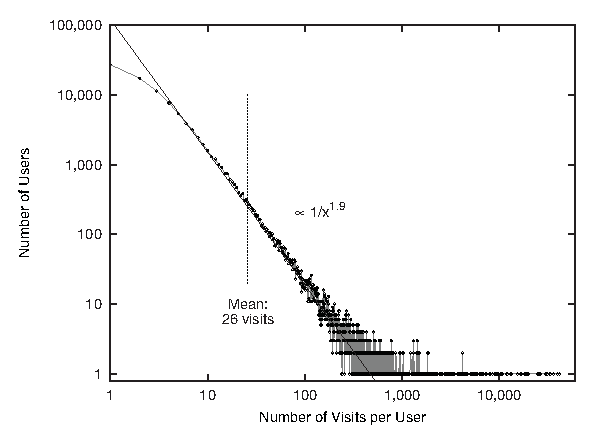
\includegraphics{img/webvisits2}}
  \caption{The data from Figure \ref{fig:webvisits1} but on double
    logarithmic scales. The righthand side of this curve is well
    described by the power law $1/x^{1.9}$.}
  \label{fig:webvisits2}
\end{figure}

Whenever they were found, power-law distributions were met with
surprise and (usually) consternation. The reason is that they possess
some unexpected and counterintuitive properties:

\begin{itemize}
\item Observations span a wide range of values, often many orders of
  magnitude.
\item There is no typical scale or value that could be used to
  summarize the distribution of points.
\item The distribution is extremely skewed, with many data points at
  the low end and few (but not negligibly few) data points at
  \emph{very} high values.
\item Expectation values often depend on the sample size. Taking the
  average over a sample of $n$ points may yield a significantly
  smaller value than taking the average over $2n$ or $10n$ data
  points.  (This is in marked contrast to most other distributions,
  where the quality of the average improves when it is based on more
  points. Not so for power-law distributions!)
\end{itemize}

It is the last item that is the most disturbing. After all, didn't the
Central Limit Theorem tell us that the scatter of the average was
always reduced by a factor of $1/\sqrt{n}$ as the sample size
increases? Yes, but remember the caveat at the end of the last
section: the Central Limit Theorem \index{Central Limit Theorem!power-law distributions} applies only to those distributions
that have a finite mean and standard deviation. For power-law
distributions, this condition is not necessarily fulfilled, and hence
the Central Limit Theorem does \emph{not} apply.

The importance of this fact cannot be overstated. Not only does much of our
intuition go out the window but most of statistical theory, too!
For the most part, distributions without expectations are simply not
treated by standard probability theory and statistics.\footnote{The
  comment on page 48 (out of 440) of Larry Wasserman's excellent
  \emph{All of Statistics} is typical: ``From now on, whenever we
  discuss expectations, we implicitly assume that they exist.''}

\subsection{Working with Power-Law Distributions}

So what should you do when you encounter a situation described by a
power-law distribution? The most important thing is to \emph{stop
  using classical methods}. In particular, the mean-field approach
(replacing the distribution by its mean) is no longer applicable and
will give misleading or incorrect results.

From a practical point of view, you can try segmenting the data (and,
by implication, the system) into different groups: the majority of
data points at small values (on the lefthand side in Figure
\ref{fig:webvisits2}), the\vadjust{\pagebreak} set of data points in the tail of the
distribution (for relatively large values), and possibly even a group
of data points making up the intermediate regime. Each such group is
now more homogeneous, so that standard methods may apply. You will
need insight into the business domain of the data, and you should
exercise discretion when determining where to make those cuts, because
the data itself will not yield a natural ``scale'' or other quantity
that could be used for this purpose.

There is one more practical point that you should be aware of when
working with power-law distributions: the form $\sim 1/x^\beta$ is
only valid ``asymptotically'' for large values of $x$. For small $x$,
this rule must be supplemented, since it obviously cannot hold for $x
\to 0$ (we can't divide by zero). There are several ways to augment
the original form near $x=0$. We can either impose a minimum value
$x_{\text{\scriptsize min}}$ of $x$ and consider the distribution only for values
larger than this. That is often a reasonable approach because such a
minimum value may exist naturally. For example there is an obvious
``minimum'' number of pages (\ie, one page) that a website visitor can
view and still be considered a ``visitor.'' Similar considerations
hold for the population of a city and the copies of books sold---all
are limited on the left by $x_{\text{\scriptsize min}} = 1$. Alternatively, the
behavior of the observed distribution may be different for small
values. Look again at Figure \ref{fig:webvisits2}: for values less
than about 5, the curve deviates from the power-law behavior that we
find elsewhere.

Depending on the shape that we require near zero, we can modify the
original rule in different ways. Two examples stand out: if we want a
flat peak for $x=0$, then we can try a form like $\sim 1/(a+x^\beta)$
for some $a>0$, and if we require a peak at a nonzero location, we can
use a distribution like $\sim \exp(-C/x)/x^\beta$ (see Figure
\ref{fig:levy}). For specific values of $\beta$, two distributions of
this kind have special names:\vspace*{-3pt}
\begin{gather*}
\frac{1}{\pi} \frac{1}{1+x^2} \quad \text{Cauchy distribution} \\
\sqrt{\frac{c}{2 \pi}} \frac{ e^{-c/2x} }{ x^{3/2} } 
                              \quad \text{L\'evy distribution}
\end{gather*}

\begin{figure}
\centerline{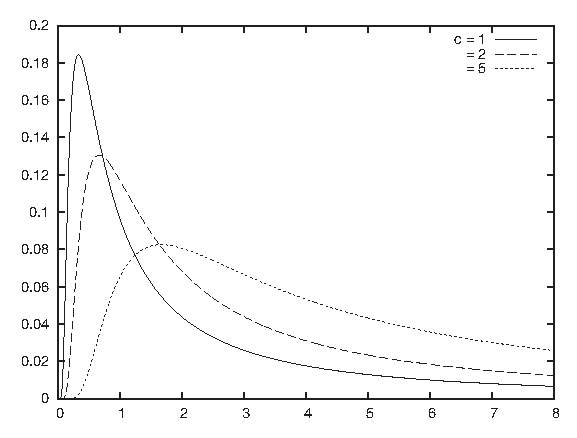
\includegraphics{img/levy}}
  \caption{The L\'evy distribution for several values of the parameter
    $c$.}
  \label{fig:levy}
\end{figure}

\vspace*{-15pt}
\subsection{Optional: Distributions with Infinite Expectation Values}

\index{infinite expectation values, distributions}
\index{expectation values!distributions with infinite expectation values} 
 
The \emph{expectation value} $E(f)$ of a function $f(x)$, which in
turn depends on some random quantity $x$, is nothing but the weighted
average of that function in which we use the probability density
$p(x)$ of $x$ as the weight function:\vspace*{-2pt}
%
\[
E(f) = \int\! f(x) p(x) \, \rms{x}
\]

Of particular importance are the expectation values for simple powers
of the variable $x$, the so called \emph{moments} of the distribution:\vspace*{-3pt}
\begin{align*}
E(1) & = \int p(x)      \, \rms{x} \quad & \text{(must always equal $1$)} \\
E(x) & = \int x \, p(x) \, \rms{x} \quad & \text{Mean or first moment} \\
E(x^2) & = \int x^2 p(x) \, \rms{x} \quad & \text{Second moment} 
\end{align*}

The first expression must always equal $1$, because we expect
$p(x)$ to be properly normalized. The second is the familiar mean,
as the weighted average of $x$. The last expression is used in the
definition of the standard deviation:
%
\[
\sigma = \sqrt{ E(x^2) - E(x)^2 }
\]
%

For power-law distributions, which behave as $\sim 1/x^\beta$ with
$\beta > 1$ for large $x$, some of these integrals may not
converge---in this case, the corresponding moment ``does not exist.''
Consider the $k$th moment ($C$ is the normalization constant $C = E(1)
= \int p(x) \, \rms{x}$):
\begin{align*}
E(x^k) & = C \int^\infty x^k \frac{1}{x^\beta} \, \rms{x} \\
       & = C \int^\infty \frac{1}{x^{\beta-k}} \, \rms{x} 
\end{align*}

Unless $\beta-k > 1$, this integral does not converge at the upper
limit of integration. (I assume that the integral is proper at the
lower limit of integration, through a lower cutoff $x_{\text{\scriptsize min}}$ or
another one of the methods discussed previously.) In particular, if
$\beta < 2$, then the mean and all higher moments do not exist; if
$\beta < 3$, then the standard deviation does not exist.

We need to understand that this is an analytical result---it tells us
that the distribution is ill behaved and that, for instance, the
Central Limit Theorem does not apply in this case. Of course, for any
\emph{finite} sample of $n$ data points drawn from such a
distribution, the mean (or other moment) will be perfectly finite. But
these analytical results warn us that, if we continue to draw
additional data points\vadjust{\pagebreak} from the distribution, then their average (or
other moment) will not settle down: it will grow as the number of data
points in the sample grows. Any summary statistic calculated from a
finite sample of points will therefore not be a good estimator for the
true (in this case: infinite) value of that statistic. This poses an
obvious problem because, of course, all practical samples contain only
a finite number of points.

Power-law distributions have no parameters that could (or need be)
estimated---except for the exponent, which we know how to obtain from
a double logarithmic plot. There is also a maximum likelihood
estimator for the exponent:
%
\[
\beta = 1 + \frac{n}{\sum_{i=0}^n \log\frac{x_i}{x_0} }
\]
%
where $x_0$ is the smallest value of $x$ for which the asymptotic
power-law behavior holds.

\subsection{Where to Go from Here}

If you want to dig deeper into the theory of heavy-tail phenomena, you
will find that it is a mess. There are two reasons for that: on the
one hand, the material is technically hard (since one must make do
without two standard tools: expectation values and the Central Limit
Theorem), so few simple, substantial, powerful results have been
obtained---a fact that is often covered up by excessive formalism. On
the other hand, the ``colorful'' and multi disciplinary context in
which power-law distributions are found has led to much confusion.
Similar results are being discovered and re-discovered in various
fields, with each field imposing its own terminology and methodology,
thereby obscuring the mathematical commonalities.

The unexpected and often almost paradoxical consequences of power-law
behavior also seem to demand an explanation for \emph{why} such
distributions occur in practice and whether they might all be
expressions of some common mechanisms. Quite a few theories have been
proposed toward this end, but none has found widespread acceptance or
proved particularly useful in predicting new phenomena---occasionally
grandiose claims to the contrary notwithstanding.

At this point, I think it is fair to say that we don't understand
heavy-tail phenomena: not when and why they occur, nor how to handle
them if they do.

% Much of the literature on power-law distributions is concerned with
% determining whether a given data set exactly follows a power-law, and
% what the best estimate for the exponent is. From a practical point of
% view, this is of no use: 

% complementary cumulative distribution function

\index{probability models!power-law distributions|)} 
\index{power-law distributions!non-normal statistics|)} 
\index{non-normal statistics and power-law distributions|)}
\index{distributions!power-law distributions|)}

% ============================================================
\section{Other Distributions}

There are some other distributions that describe common scenarios you
should be aware of. Some of the most important (or most frequently
used) ones are described in this section.

\subsection{Geometric Distribution}

\index{probability models!geometric distribution}
\index{distributions!geometric distribution}
\index{geometric distribution}
   
The geometric distribution (see Figure \ref{fig:geometric}):
%
\[
p( k, p ) = p (1-p)^{k-1} \quad \text{with $k = 1, 2, 3, \dots$}
\]
%
is a special case of the binomial distribution. It can be viewed as
the probability of obtaining the first Success at the $k$th trial
(\ie, after observing $k-1$ failures). Note that there is only a
single arrangement of events for this outcome, hence the combinatorial
factor is equal to one. The geometric distribution has mean $\mu =
1/p$ and standard deviation $\sigma = \sqrt{1-p}/p$.

\begin{figure}
\centerline{ 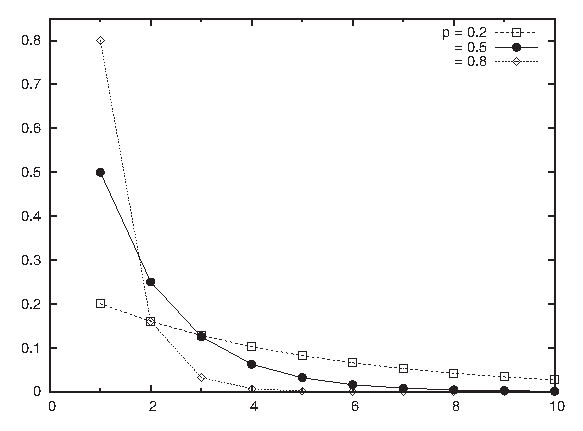
\includegraphics{img/geometric}}
  \caption{The geometric distribution: $p( k, p ) = p (1-p)^{k-1}$.}
  \label{fig:geometric}
\end{figure}


\subsection{Poisson Distribution}

\index{probability models!Poisson distribution}
\index{distributions!Poisson distribution}
\index{Poisson distribution}

The binomial distribution gives us the probability of observing
exactly $k$ events in $n$ distinct trials. In contrast, the Poisson
distribution describes the probability of finding $k$ events during
some continuous observation \emph{interval} of known length.  Rather
than being characterized by a probability parameter and a number of
trials (as for the binomial distribution), the Poisson distribution is
characterized by a \emph{rate} $\lambda$ and an \emph{interval length}
$t$.

The Poisson distribution $p(k,t,\lambda)$ gives the probability of
observing exactly $k$ events during an interval of length $t$ when the
rate at which events occur is $\lambda$ (see Figure
\ref{fig:poisson}):
%
\[
p(k, t, \lambda) = \frac{(\lambda t)^k}{k!} e^{-\lambda t}
\]
%
Because $t$ and $\lambda$ only occur together, this expression is
often written in a two-parameter form as $p(k, \nu) = e^{-\nu}
\nu^k/k!$. Also note that the term $e^{-\lambda t}$ does not depend on
$k$ at all---it is merely there as a normalization factor. All the
action is in the fractional part of the equation.

\begin{figure}
\centerline{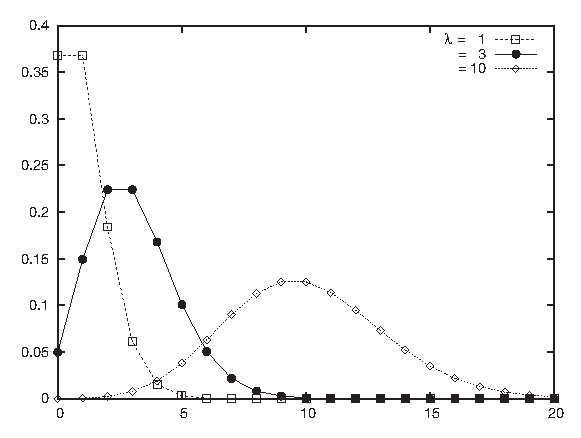
\includegraphics{img/poisson}}
  \caption{The Poisson distribution: 
    $p(k, t, \lambda) = \frac{(\lambda t)^k}{k!} e^{-\lambda t}$.}
  \label{fig:poisson}
\end{figure}

Let's look at an example.  Assume that phone calls arrive at a call
center at a rate of 15 calls per hour (so that $\lambda = 0.25\,
\text{calls}/\text{minute}$). Then the Poisson distribution $p(k, 1,
0.25)$ will give us the probability that $k=0,1,2,\dots$ calls will
arrive in any given minute. But we can also use it to calculate the
probability that $k$ calls will arrive during any 5-minute time
period: $p(k, 5, 0.25)$.  Note that in this context, it makes no sense
to speak of independent trials: time passes continuously, and the
expected number of events depends on the length of the observation
interval.

We can collect a few results. Mean $\mu$ and standard deviation 
$\sigma$ for the Poisson distribution are given by:
\begin{align*}
\mu    & = \lambda t \\
\sigma & = \sqrt{ \lambda t }
\end{align*}

Notice that only a single parameter ($\lambda t$) controls both the
location and the width of the distribution. For large $\lambda$, the
Poisson distribution approaches a Gaussian distribution with $\mu =
\lambda$ and $\sigma = \sqrt{\lambda}$. Only for small values of
$\lambda$ (say, $\lambda < 20$) are the differences notable.

Conversely, to estimate the parameter $\lambda$ from observations, we
divide the number $k$ of events observed by the length\vadjust{\pagebreak} $t$ of the
observation period: $\lambda = k/t$.  Keep in mind that when
evaluating the formula for the Poisson distribution, the rate
$\lambda$ and the length $t$ of the interval of interest must be of
compatible units.  To find the probability of $k$ calls over 6 minutes
in our call center example above, we can either use $t=6\,
\text{minutes}$ and $\lambda = 0.25\, \text{calls per minute}$ or
$t=0.1\, \text{hours}$ and $\lambda = 15\, \text{calls per hour}$, but
we cannot mix them. (Also note that $6 \cdot 0.25 = 0.1 \cdot 15 =
1.5$, as it should.)

The Poisson distribution is appropriate for processes in which
discrete events occur independently and at a constant rate: calls to a
call center, misprints in a manuscript, traffic accidents, and so on.
However, you have to be careful: it applies only if you can identify a
rate at which events occur \emph{and} if you are interested
specifically in the number of events that occur during intervals of
varying length.  (You cannot expect every histogram to follow a
Poisson distribution just because ``we are counting events.'')


\subsection{Log-Normal Distribution}

\index{probability models!log-normal distribution}
\index{distributions!log-normal distribution}
\index{log-normal distribution}

Some quantities are inherently asymmetrical. Consider, for example,
the time it takes people to complete a certain task: because
everyone is different, we expect a distribution of values. However,
all values are necessarily positive (since times cannot be negative).
Moreover, we can expect a particular shape of the distribution: there
will be some minimum time that nobody can beat, then a small group of
very fast champions, a peak at the most typical completion time, and
finally a long tail of stragglers. Clearly, such a distribution will
not be well described by a Gaussian, which is defined for both
positive and negative values of $x$, is symmetric, and has short
tails!

The log-normal distribution is an example of an asymmetric
distribution that is suitable for such cases. It is related to the
Gaussian: a quantity follows the log-normal distribution if its
logarithm is distributed according to a Gaussian.

The probability density for the log-normal distribution looks
like this:
%
\[
p(x; \mu, \sigma ) = \frac{1}{\sqrt{2\pi}\sigma x}
                     \exp \paren{- \frac{1}{2} 
                          \paren{ \frac{\log(x/\mu)}{\sigma} }^2 }
\]
%
(The additional factor of $x$ in the denominator stems from the
Jacobian in the change of variables from $x$ to $\log x$.)  You may
often find the log-normal distribution written slightly differently:
%
\[
p(x; \tilde{\mu}, \sigma ) = \frac{1}{\sqrt{2\pi}\sigma x}
                \exp \paren{- \frac{1}{2} 
                     \paren{ \frac{\log(x) - \tilde{\mu}}{\sigma} }^2 }
\]
%
This is the same once you realize that $\log(x/\mu) = \log(x) -
\log(\mu)$ and make the identification $\tilde{\mu} = \log(\mu)$.  The
first form is much better because it expresses clearly that $\mu$ is
the \emph{typical scale} of the problem. It also ensures that the
argument of the logarithm is dimensionless (as it must be).

\begin{figure}
 \centerline{ 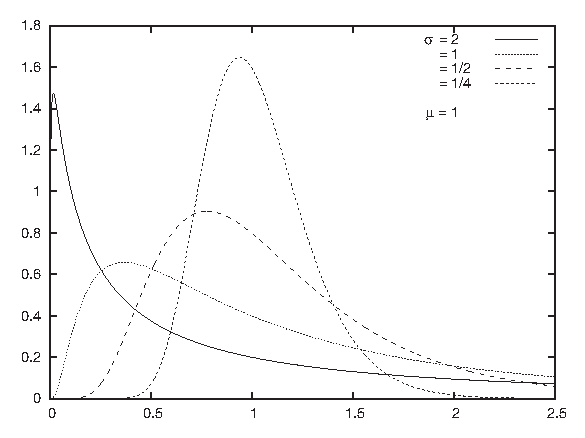
\includegraphics{img/lognormal}}
  \caption{The log-normal distribution.}
  \label{fig:lognormal}
\end{figure}\pagebreak

Figure \ref{fig:lognormal} shows the log-normal distribution for a few
different values of $\sigma$. The parameter $\sigma$ controls the
overall ``shape'' of the curve, whereas the parameter $\mu$ controls
its ``scale.'' In general, it can be difficult to predict what the
curve will look like for different values of the parameters, but here
are some results (the \emph{mode} is the position of the peak).
\begin{align*}
\text{Mode:} \quad & \mu e^{-\sigma^2} \\
\text{Mean:} \quad & \mu e^{\frac{\sigma^2}{2}} \\
\text{Standard deviation:} \quad & 
                     \mu \sqrt{e^{\sigma^2} \paren{ e^{\sigma^2} - 1 }}
\end{align*}

Values for the parameters can be estimated from a data set as follows:
\begin{align*}
\mu    & = \exp \paren{\frac{1}{n} \sum_{i=1}^n \log x_i} \\
\sigma & = \sqrt{ \frac{1}{n} \sum_{i=1}^n \paren{\log\frac{x_i}{\mu}}^2}
\end{align*}

The log-normal distribution is important as an example of a standard
statistical distribution that provides an alternative to the Gaussian
model for situations that require an asymmetrical distribution.  That
being said, the log-normal distribution can be fickle to use in
practice. Not all asymmetric point distributions are described well by
a log-normal distribution, and you may not be able to obtain a good
fit for your data using a log-\break normal distribution.  For truly
heavy-tail phenomena in particular, you will need a power-law
distribution after all.  Also keep\vadjust{\pagebreak} in mind that the log-normal
distribution approaches the Gaussian as $\sigma$ becomes small
compared to $\mu$ (\ie, $\sigma/\mu \ll 1$), at which point it becomes
easier to work with the familiar Gaussian directly.


\subsection{Special-Purpose Distributions}

\index{probability models!special-purpose distributions}
\index{distributions!special-purpose distributions}
 
Many additional distributions have been defined and studied. Some,
such as the gamma distribution, are mostly of theoretical importance,
whereas others---such as the chi-square, $t$, and $F$
distributions---are are at the core of classical, frequentist
statistics (we will encounter them again in Chapter
\ref{ch:statistics}). Still others have been developed to model
specific scenarios occurring in practical applications---especially in
reliability engineering, where the objective is to make predictions
about likely failure rates and survival times.

I just want to mention in passing a few terms that you may encounter.
The \emph{Weibull} distribution is used to express the probability
that a device will fail after a certain time. Like the log-normal
distribution, it depends on both a shape and a scale parameter.
Depending on the value of the shape parameter, the Weibull
distribution can be used to model different failure modes. These
include ``infant mortality'' scenarios, where devices are more likely
to fail early but the failure rate declines over time as defective
items disappear from the population, and ``fatigue death'' scenarios,
where the failure rate rises over time as items age.

Yet another set of distributions goes by the name of
\emph{extreme-value} or \emph{Gumbel} distributions. They can be used
to obtain the probability that the smallest (or largest) value of some
random quantity will be of a certain size. In other words, they answer
the question: what is the probability that the largest element in a
set of random numbers is precisely $x$?

Quite intentionally, I don't give formulas for these distributions
here. They are rather advanced and specialized tools, and if you want
to use them, you will need to consult the appropriate references.
However, the important point to take away here is that, for many
typical scenarios involving random quantities, people have developed
explicit models and studied their properties; hence a little research
may well turn up a solution to whatever your current problem is.


% ============================================================
\section{Optional: Case Study�Unique Visitors over Time}

\index{probability models!Unique Visitors over Time case study|(} 
\index{Unique Visitors over Time case study|(}
 
To put some of the ideas introduced in the last two chapters into
practice, let's look at an example that is a bit more involved. We
begin with a probabilistic argument and use it to develop a mean-field
model, which in turn will lead to a differential equation that we
proceed to solve for our final answer.  This example demonstrates how
all the different ideas we have been introducing in the last few
chapter can fit together to tackle more complicated problems.

Imagine you are running a website.  Users visit this website every day
of the month at a rate that is roughly constant.  We can\vadjust{\pagebreak} also assume
that we are able to track the identity of these users (through a
cookie or something like that). By studying those cookies, we can see
that some users visit the site only once in any given month while
others visit it several times. We are interested in the number of
\emph{unique users} for the month and, in particular, how this number
develops over the course of the month. (The number of unique visitors
is a key metric in Internet advertising, for instance.)

The essential difficulty is that some users visit several times during
the month, and so the number of unique visitors is smaller than the
total number of visitors. Furthermore, we will observe a ``saturation
effect'': on the first day, almost every user is new; but on the last
day of the month, we can expect to have seen many of the visitors
earlier in the month already.

We would like to develop some understanding for the number of unique
visitors that can be expected for each day of the month (\eg, to
monitor whether we are on track to meet some monthly goal for the
number of unique visitors). To make progress, we need to develop a
model.

To see more clearly, we use the following idealization, which is
equivalent to the original problem. Consider an urn that contains $N$
identical tokens (total number of potential visitors). At each turn
(every day), we draw $k$ tokens randomly from the urn (average number
of visitors per day). We mark all of the drawn tokens to indicate that
we have ``seen'' them and then place them back into the urn.  This
cycle is repeated for every day of the month.

Because at each turn we mark all unmarked tokens from the random
sample drawn at this turn, the number of marked tokens in the urn will
increase over time. Because each token is marked at most once, the
number of marked tokens in the urn at the end of the month is the
number of unique visitors that have visited during that time period.

Phrased this way, the process can be modeled as a sequence of
Bernoulli trials. We define drawing an already marked token as
Success. Because the number of marked tokens in the urn is increasing,
the success probability $p$ will change over time. The relevant
variables are:
\begin{align*}
N    & \quad \text{Total number of tokens in urn} \\
k    & \quad \text{Number of tokens drawn at each turn} \\
m(t) & \quad \text{Number of already-marked tokens drawn at turn $t$} \\
n(t) & \quad \text{Total number of marked tokens in urn at time $t$} \\
p(t) = \frac{n(t)}{N} & \quad \text{Probability of drawing an already-marked token at turn $t$}
\end{align*}

Each day consists of a new Bernoulli trial in which $k$ tokens are
drawn from the urn. However, because the number of marked tokens in
the urn increases every day, the probability $p(t)$ is different every
day.

On day $t$, we have $n(t)$ marked tokens in the urn. We now draw $k$
tokens, of which we expect $m(t) = k p(t)$ to be marked (Successes).
This is simply an application of the basic result for the expectation
value of Bernoulli trials, using the current value for the
probability. (Working with the expectation value in this way
constitutes a mean-field approximation.)

The number of unmarked tokens in the current drawing is:
%
\[
k - m(t) = k - k p(t) = k ( 1 - p(t) )
\]
%
We now mark these tokens and place them back into the urn, which means
that the number of marked tokens in the urn grows by $k(1-p(t))$:
%
\[
n(t+1) = n(t) + k ( 1 - p(t) )
\]
%
This equation simply expresses the fact that the new number of marked
tokens $n(t+1)$ consists of the previous number of marked tokens
$n(t)$ \emph{plus} the newly marked tokens $k(1-p(t))$.

We can now divide both sides by $N$ (the total number of tokens).
Recalling that $p(t) = n(t)/N$, we write:
%
\[
p(t+1) = p(t) + f( 1 - p(t) ) \quad \text{with } f = \frac{k}{N}
\]
%
This is a recurrence relation for $p(t)$, which can be rewritten as:
%
\[
p(t+1) - p(t) = f( 1 - p(t) )
\]

In the continuum limit, we replace the difference between the
``new'' and the ``old'' values by the \emph{derivative} at time
$t$, which turns the recurrence relation into a more convenient
differential equation:
%
\[
\frac{\text{d}p(t)}{\text{d}t} = f ( 1 - p(t) )
\]
%
with initial condition $p(t=0) = 0$ (because initially there are no
marked tokens in the urn). This differential equation has the
solution:
%
\[
p(t) = 1 - e^{-ft}
\]

Figure \ref{fig:uniques} shows $p(t)$ for various values of the
parameter $f$.  (The parameter $f$ has an obvious interpretation as
size of each drawing expressed as a fraction of the total number of
tokens in the urn.)

\begin{figure}
\centerline{ 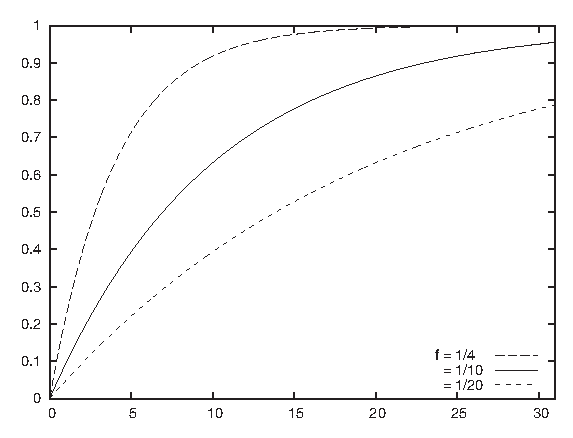
\includegraphics{img/uniques}}
  \caption{Fraction of unique visitors seen on day $t$. The parameter
    $f$ is the number of daily users expressed as a fraction of all
    potential users.}
  \label{fig:uniques}
\end{figure}

This is the result that we have been looking for. Remember that $p(t)
= n(t)/N$; hence the probability is directly proportional to the
number of unique visitors so far. We can rewrite it more explicitly as:
%
\[
n(t) = N \paren{ 1 - e^{ -\frac{k}{N} t} }
\]
%
In this form, the equation gives us, for each day of the month, the
number of unique visitors for the month up to that date. There is only
one unknown parameter: $N$, the total number of \emph{potential}
visitors. (We know $k$, the average number of total visitors per day,
because this number is immediately available from the web-server
logs.)  We can now try to fit one or two months' worth of data to this
formula to obtain a value for $N$. Once we have determined $N$, the
formula predicts the expected number of unique visitors for each day
of the month. We can use this information to track whether the actual
number of unique visitors for the current month is above or below
expectations.

The steps we took in this little example are typical of a lot of
modeling. We start with a real problem in a specific situation.  To
make headway, we recast it in an idealized format that tries to retain
only the most relevant information.  (In this example: mapping the
original problem to an idealized urn model.) Expressing things in
terms of an idealized model helps us recognize the problem as one we
know how to solve. (Urn models have been studied extensively; in this
example, we could identify it with Bernoulli trials, which we know how
to handle.) Finding a solution often requires that we make actual
approximations in addition to the abstraction from the problem domain
to an idealized model. (Working with the expectation value was one
such approximation to make the problem tractable; replacing the
recurrence relation with a differential equation was another.)
Finally, we end up with a ``model'' that involves some unknown
parameters. If we are mostly interested in developing conceptual
understanding, then we don't need to go any further, since we can read
off the model's\vadjust{\pagebreak} behavior directly from the formula.  However, if we
actually want to make numerical predictions, then we'll need to find
numerical values for those parameters, which is usually done by
fitting the model to some already available data. (We should also try
to validate the model to see whether it gives a good ``fit''; refer to
the discussion in Chapter \ref{ch:bivariate} on examining residuals,
for instance.)

Finally, I should point out that the model in this example is
simplified---as models usually are. The most critical simplification
(which would most likely \emph{not} be correct in a real application)
is that every token in the urn has the same probability of being drawn
at each turn.  In contrast, if look at the behavior of actual
visitors, we will find that some are much more likely to visit more
frequently while others are less likely to visit. Another
simplification is that we assumed the total number of potential
visitors to be constant. But if we have a website that sees
significant growth from one month to the next, this assumption may not
be correct, either. You may want to try and build an improved model
that takes these (and perhaps other) considerations into account. (The
first one in particular is not easy---in fact, if you succeed, then
let me know how you did it!)

\index{probability models!Unique Visitors over Time case study|)} 
\index{Unique Visitors over Time case study|)}

% ============================================================
\section{Workshop: Power-Law Distributions}

\index{probability models!power-law distributions} 
\index{distributions!power-law distributions}
\index{power-law distributions!example}  
 
The crazy effects of power-law distributions have to be seen to be
believed. In this workshop, we shall generate (random) data points
distributed according to a power-law distribution and begin to study
their properties.

First question: how does one actually generate nonuniformly
distributed random numbers on a computer? A random generator that
produces uniformly distributed numbers is available in almost all
programming environments, but generating random numbers distributed
according to some other distribution requires a little bit more work.
There are different ways of going about it; some are specific to
certain distributions only, whereas others are designed for speed in
particular applications. We'll discuss a simple method that works for
distributions that are analytically known.

The starting point is the cumulative distribution function for the
distribution in question. By construction, the distribution function
is strictly monotonic and takes on values in the interval $[0,1]$. If
we now generate uniformly distributed numbers between 0 and 1, then we
can find the locations at which the cumulative distribution function
assumes these values. These points will be distributed according to
the desired distribution (see Figure \ref{fig:randomnums}).

\begin{figure}
\centerline{ 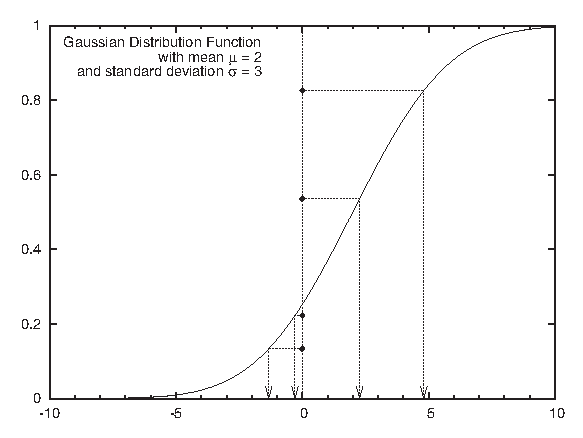
\includegraphics{img/randomnums}}
  \caption{Generating random numbers from the Gaussian distribution:
    generate uniformly distributed numbers between $0$ and $1$, then
    find the locations values at which the Gaussian distribution
    function assumes these values. The locations follow a Gaussian
    distribution.}
  \label{fig:randomnums}
\end{figure}

(A good way to think about this is as follows. Imagine you distribute
$n$ points \emph{uniformly} on the interval $[0,1]$ and find the
corresponding locations at which the cumulative distribution function
assumes these values. These locations are spaced according to the
distribution in question---after all, by construction, the
probability grows by the same amount between successive locations.
Now use points that are randomly distributed, rather than uniformly,
and you end up with random points distributed according to the
desired distribution.)

For power-law distributions, we can easily work out the cumulative
distribution function and its inverse. Let the probability density
$p(x)$ be:
%
\[
p(x) = \frac{\alpha}{x^{\alpha+1}} \quad x \ge 1, \alpha > 0
\]
%
This is known as the the ``standard'' form of the Pareto distribution.\index{Pareto distribution, standard form}
It is valid for values of $x$ greater than $1$. (Values of $x<1$ have
zero probability of occurring.) The parameter $\alpha$ is the ``shape
parameter'' and must be greater than zero, because otherwise the
probability is not normalizable. (This is a different convention than
the one we used earlier: $\beta = 1 + \alpha$.)

We can work out the cumulative distribution function $P(x)$:
%
\begin{align*}
P(x) = y & = \int_1^x p(t) \rms{t} \\
         & = 1 - \frac{1}{x^\alpha}
\end{align*}
%
This expression can be inverted to give:
%
\[
x = \frac{1}{(1-y)^{1/\alpha}}
\]
%
If we now use uniformly distributed random values for $y$, then the
values for $x$ will be distributed according to the Pareto
distribution that we started with. (For other distributions, such as
the Gaussian, inverting the expression for the cumulative distribution
function is often harder, and you may have to find a numerical library
that includes the inverse of the distribution function explicitly.)

Now remember what we said earlier. If the exponent in the denominator
is less than 2 (\ie, if $\beta \le 2$ or $\alpha \le 1$), then the
``mean does not exist.'' In practice, we can evaluate the mean for any
sample of points, and for any \emph{finite} sample the mean will, of
course, also be finite.  But as we take more and more points, the mean
does not settle down---instead it keeps on growing. On the other hand,
if the exponent in the denominator is strictly greater than 2 (\ie, if
$\beta > 2$ or $\alpha > 1$), then the mean does exist, and its value
does not depend on the sample size.

I would like to emphasize again how counterintuitive the behavior for
$\alpha \le 1$ is. We usually expect that larger samples will give us
better results with less noise. But in this particular scenario, the
opposite is true!

We can explore behavior of this type using the simple program shown
below.  All it does is generate 10 million random numbers distributed
according to a Pareto distribution. I generate those numbers using the
method described at the beginning of this section; alternatively, I
could have used the \texttt{paretovariate()} function in the standard
\texttt{random} module. We maintain a running total of all values (so
that we can form the mean) and also keep track of the largest value
seen so far. The results for two runs with $\alpha = 0.5$ and $\alpha
= 1.2$ are shown in Figures \ref{fig:pareto1} and \ref{fig:pareto2},
respectively.

\begin{verbatim}
import sys, random

def pareto( alpha ):
    y = random.random()
    return 1.0/pow( 1-y, 1.0/alpha )


alpha = float( sys.argv[1] )

n, ttl, mx = 0, 0, 0

while n<1e7:
    n += 1

    v = pareto( alpha )

    ttl += v
    mx = max( mx, v )
    
    if( n%50000 == 0 ):
        print n, ttl/n, mx
\end{verbatim}

The typical behavior for situations with $\alpha \le 1$ versus $\alpha
> 1$ is immediately apparent: whereas in Figure \ref{fig:pareto2}, the
mean settles down pretty quickly to a finite value, the mean in Figure
\ref{fig:pareto1} continues to grow.

\begin{figure}
\centerline{ 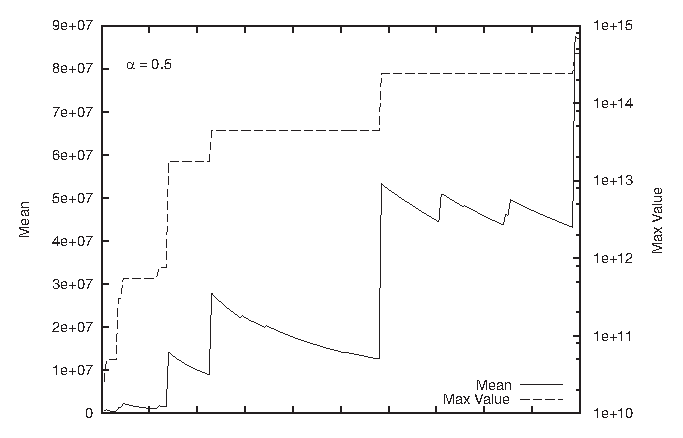
\includegraphics{img/pareto1}}
  \caption{Sampling from the Pareto distribution $P(x) = \frac{1}{2
      x^{3/2}}$. Both the mean and the maximum value grow without
    bound.}
  \label{fig:pareto1}
\end{figure}

We can also recognize clearly what drives this behavior. For $\alpha
\le 1$, very large values occur relatively frequently. Each such
occurrence leads to an upward jump in the total sum of values seen,
which is reflected in a concomitant jump in the mean. Over time, as
more trials are conducted, the denominator\vadjust{\pagebreak} in the mean grows, and hence
the value of the mean begins to fall. However (and this is what is
different for $\alpha \le 1$ versus $\alpha > 1$), before the mean has
fallen back to its previous value, a \emph{further} extraordinarily
large value occurs, driving the sum (and hence the mean) up again,
with the consequence that the numerator of the expression
\texttt{ttl/n} in the example program grows faster than the
denominator.

You may want to experiment yourself with this kind of system. The
behavior at the borderline value of $\alpha = 1$ is particularly
interesting. You may also want to investigate how quickly
\texttt{ttl/n} grows with different values of $\alpha$. Finally, don't
restrict yourself only to the mean.  Similar considerations hold for
the standard deviation (see our discussion regarding this point
earlier in the chapter).


\begin{figure}
\centerline{ 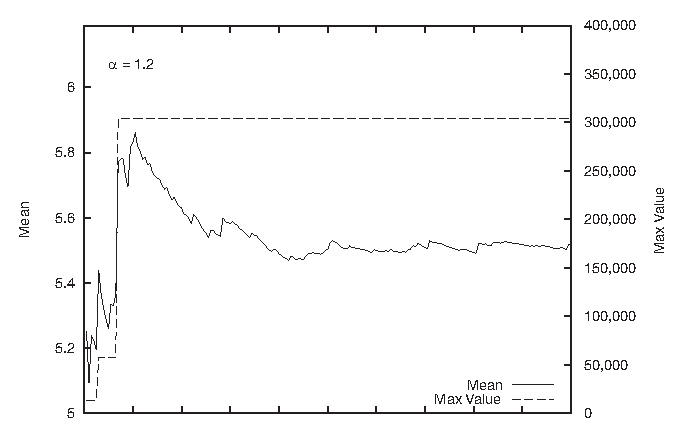
\includegraphics{img/pareto2}}
  \caption{Sampling from the Pareto distribution $P(x) =
    \frac{1.2}{x^{2.2}}$. Both the mean and the maximum reach a finite
    value and retain it as we continue to make further drawings.}
  \label{fig:pareto2}
\end{figure}

% ============================================================
\section{Further Reading}

\begin{itemize}
\item \cit{An Introduction to Probability Theory and Its Applications,
    vol. 1}{William Feller}{3rd ed., Wiley}{1968} 
  Every introductory book on probability theory covers most of the
  material in this chapter. This classic is my personal favorite for
  its deep, yet accessible treatment and for its large selection of
  interesting or amusing examples.

\item \cit{An Introduction to Mathematical Statistics and Its
    Applications}{Richard J.\ Larsen and Morris L.\ Marx}{4th ed.,
    Prentice Hall}{2005}
  This is my favorite book on theoretical statistics. The first third
  contains a good, practical introduction to many of this chapter's
  topics.

\item \cit{NIST/SEMATECH e-Handbook of Statistical
    Methods}{NIST}{\url{http://www.itl.nist.gov/div898/handbook/}}{2010}
  This free ebook is made available by the National Institute for 
  Standards and Technology (NIST). There is a wealth of reliable,
  high-quality information here.

\item \cit{Statistical Distributions}{Merran Evans, Nicholas Hastings,
    and Brian Peacock}{3rd ed., Wiley}{2000}
  This short and accessible reference includes basic information on
  40 of the most useful or important probability distributions. If 
  you want to know what distributions exist and what their properties
  are, this is a good place to start.

\item \pcit{Power Laws, Pareto Distributions and Zipf's Law}{M.\ E.\
    J.\ Newman}{Contemporary Physics}{46}{2005}{323} \\
  This review paper provides a knowledgeable yet very readable
  introduction to the field of power laws and heavy-tail phenomena.
  Highly recommended. (Versions of the document can be found on the
  Web.)

\item \cit{Modeling Complex Systems}{Nino Boccara}{2nd ed., Springer}{2010}  
  Chapter 8 of this book provides a succinct and level-headed overview
  of the current state of research into power-law phenomena. 
%(A second
%  edition of is expected in late 2010.)
\end{itemize}

\index{data analysis!probability models|)} 
\index{probability models|)}
\index{distributions|)} 


\clearpage

\thispagestyle{empty}

\cleardoublepage